\chapter{一种孤立中心损失方法及其在分类任务中的应用}


\section{引言}

分心驾驶行为检测归属于分类任务,然而所有的分类任务都遵循一个共同原则,即特征的区分度(Discrimination)越高越好,在分类任务中,样本类别之间的区分度尽可能区分明显。

Softmax损失函数(Softmax Loss,SL)是分类任务最常用的一种监督方法,针对Softmax损失监督下各类样本之间区分度不足,提出了一种孤立中心损失监督方法。基于类间离散度尽量大、类内离散度尽量小的原则,提出方法由三部分组成:第一部分采用等角分布固定权值,使得全部类间夹角余弦值之和最小,确保不同类别在角度空间的距离最大化;第二部分是中心聚类思想,最小化每个样本与其所属类别的中心之间的欧氏距离,促使同类样本尽量聚拢;第三部分最大化不同类之间的欧氏距离,使得不同类样本在欧氏空间尽量分开。在分类数据集AUCD2、FER2013、FERPlus和RAF-DB上的测试结果显示:在分类数据集AUCD2、FER2013、FERPlus和RAF-DB上的测试结果表明:相比于Softmax损失函数,提出方法不仅提高了准确率,同时也更加稳定(相同配置下多次实验结果的变化程度更小)。提出方法的运行速度只比Softmax损失方法略微慢一点,仍然比一些其它方法快。

分心驾驶行为检测是典型的多分类问题,每一个样本必归属某一个类别,且只属于一个类别。Softmax Loss (SL)是一种交叉熵损失,经过Softmax变换,每一个样本最终输出对应多个类别的概率值(相对概率)。SL通过优化预测概率与目标概率之间的误差,会持续拉高正确类别的概率和降低错误分类的概率。在多分类问题上,SL显得直观、易理解,而且反向求导简洁,是应用最广泛的一种监督函数。

SL尽力把不同类别样本特征在角度空间分开,在SL监督下学习到的深度特征的区分度不够好\cite{57},因此,研究者们对SL进行了改进\cite{58,59,60}。针对SL的改进技术主要分两类,一类是改变SL本身(即SL的变体),即CosFace\cite{65}、ArcFace\cite{68},另一类是增加约束项协同SL一起工作,例如Center loss(CL)\cite{63,64}和Island Loss(IL)\cite{69}等。

分类任务有个共同原则,深度特征的区分度越高越好,即“类间特征分离,类内特征聚集”的指导思想。现有技术主要通过两个方面来提高特征区分度,一是减小类内距离,二是增大不同类之间的距离。


CL采用中心聚类思想,减小同类样本之间的欧式距离,有效降低类内变化。Luo等\cite{61}认为同一种表情并非高度相似,同一种表情中也应该分成几个子类,从而提出了Subcenter Loss(SCL)。Li等\cite{61,62}则减小每个样本与其相邻几个同类样本中心的距离,从而促使同类样本收敛在一起,这种方法兼具了CL和SCL的优点,但是计算复杂度高,且需要额外的内存开销。

IL在SL的基础上采用了CL,同时通过最小化不同类中心夹角的余弦值,期望不同类之间的夹角尽量大。IL需要约束每一类与其它类的夹角,难以处理类别数量多的任务,Jiang等人\cite{66}证明了类间夹角相等且等于$arccos{\left(1/\left(1-n\right)\right)}$($n$为类别数量)是类间角度距离最大化的一种理想状态,基于此提出了一种改进Softmax损失(ASL)。

ASL能够有效地最大化类间角度距离,CL能够有效地减小类内变化,但是ASL与CL单纯地协同工作(即ASL+CL)并非更优秀,可能比ASL更差(详见本章仿真)。针对以上所叙述问题,提出了一种孤立中心聚类损失(Isolated Center Loss, ICL)方法\cite{71},以ASL为基础融合中心聚类思想(即改进CL以符合ASL),再最大化类间欧式距离,使各类成为彻底的“孤岛”。实验结果表明,提出方法在识别精度和稳定性方面都有较好的提升。

\section{改进Softmax损失函数}

无偏量的SL一般定义如公式(\ref{公式4-1})所示:

\begin{equation}\label{公式4-1}
	\mathcal{L}_{SL}=-\frac{1}{m}\sum_{i=1}^{m}{log\frac{e^{\symbfit{w}_{y_i}^T\symbfit{x}_i}}{\sum_{k\in\mathbfcal{D}} e^{\symbfit{w}_k^T\symbfit{x}_i}}}
\end{equation}


其中,$\mathbfcal{D}={1,\ldots,n}$是样本类别标签集合,$\left(\cdot\right)^T$代表转置操作,$\symbfit{x}_i\in\mathbb{R}^d$表示第i个深度特征向量,$y_i\in\mathbfcal{D}$是对应的类别标签,$\symbfit{w}_k\in\mathbb{R}^d$是对应第k类的权值参数向量,SL中全体权值参数表示为$\symbfit{W}=\left[\symbfit{w}_1,\symbfit{w}_2,\ldots,\symbfit{w}_n\right]\in\mathbb{R}^{d\times n}$,$n$和$m$分别表示类别数目和训练样本数量(一批)。

一个训练理想的模型,第$k$类特征的中心就在其对应权值向量$\symbfit{w}_k$的方向上,即$\symbfit{w}_k$可以代表第$k$类中心的方向。若用$A_{kl}$表示第$k$和$l$类(中心)的夹角,则$A_{kl}$的余弦值为:

\begin{equation}\label{公式4-2}
	\cos \left(A_{k l}\right)=\frac{\symbfit{w}_{k}^{T}}{\left\|\symbfit{w}_{k}\right\|} \frac{\symbfit{w}_{l}}{\left\|\symbfit{w}_{l}\right\|}=\widehat{\symbfit{w}}_{k}^{T} \widehat{\symbfit{w}}_{l}
\end{equation}

其中,${\hat{\symbfit{w}}}_k$和${\hat{\symbfit{w}}}_l$是单位化的$\symbfit{w}_k$和$\symbfit{w}_l$,$||·||$表示向量的模。余弦值$\cos{\left(A_{kl}\right)}$越小,夹角$A_{kl}$越大。

基于类间角度距离(夹角)越大,区分度越高的原则,考虑如公式(\ref{公式4-3})所示损失函数:

\begin{equation}\label{公式4-3}
	\mathcal{L}_{Angle}=\sum_{\mathrm{k} \in \mathcal{D}} \sum_{l \in \mathcal{D}, l \neq k} \widehat{\symbfit{w}}_{k}^{T} \widehat{\symbfit{w}}_{l}
\end{equation}

$\mathcal{L}_{Angle}$是所有夹角的余弦值之和,$\mathcal{L}_{Angle}$越小表示各类之间的夹角越大,区分度越好。


深度特征维数$d\geq n-1$时,$\widehat{\symbfit{w}}_{k}^{T} \widehat{\symbfit{w}}_{l}=1 /(1-n)$可以使$\mathcal{L}_{Angle}$取得极小值$-n$(即$\mathcal{L}_{Angle}=-n$),即每个夹角$A_{k l}=\arccos (1 /(1-n))$是最小化$\mathcal{L}_{Angle}$的一种理想解。

$A_{k l}=\arccos (1 /(1-n))$仅仅是$\mathcal{L}_{Angle}=-n$的一个解,而不是唯一解,所以,通过梯度下降方法优化$\mathcal{L}_{Angle}$损失不能确保每一个夹角$A_{kl}$都满足$A_{k l}=\arccos (1 /(1-n))$。文献\cite{66}给出了一个自动生成权值参数的算法,能够保证每一个夹角$A_{k l}=\arccos (1 /(1-n))$,这是ASL的核心思想。

ASL的定义如公式(\ref{公式4-4})所示:

\begin{equation}\label{公式4-4}
		\mathcal{L}_{ASL}=-\frac{1}{m}\sum_{i=1}^{m}{log\frac{e^{\symbfit{w}_{y_i}^T\symbfit{x}_i}}{\sum_{k\in\mathbfcal{D}} e^{\symbfit{w}_k^T\symbfit{x}_i}}}  	
\end{equation}

$$
s.t. \quad \left\|\symbfit{w}_{k}\right\|=1 \quad \rm{and} \quad \symbfit{w}_{k}^{T} \symbfit{w}_{l}=\frac{1}{1-n} \cdot(k, l \in \mathcal{D})
$$

对比公式(\ref{公式4-4})和公式(\ref{公式4-4}),ASL只是对SL的权值做了限制。ASL在初始化时,权值向量$\symbfit{w}_k$由文献\cite{66}的算法1生成,在训练时固定不变。

ASL的优势有两点:(1)ASL的权值向量等角度分布,可以缓解多样本类容易挤压少样本类角度空间的问题,在一定程度上可以解决样本不平衡的问题;(2)ASL采用的迭代初始化权重,不再更新权重,所以ASL的训练速度比SL快。

\section{CenterLoss损失函数}

针对SL只注重类间差异,忽略类内差异性过大的问题,文献\cite{64}提出了一个减小类内离散度的约束函数,即著名的中心聚类损失函数(CL),其定义如公式(\ref{公式4-5})所示:

\begin{equation}\label{公式4-5}
	\mathcal{L}_{C L}=\frac{1}{2 m} \sum_{i=1}^{m}\left\|\symbfit{x}_{i}-\symbfit{c}_{y_{i}}\right\|^{2}
\end{equation}

其中$\symbfit{c}_{y_i}$表示第$y_i$类的中心。

CL是对SL的一种辅助,与SL一起监督学习,学习时总损失可以表示为:

\begin{equation}\label{公式4-6}
	\mathcal{L}=\mathcal{L}_{SL}{+\lambda\mathcal{L}}_{CL}
\end{equation}


$\lambda$是一个权值,决定了CL约束效果。$\lambda=0$时,CL无效;$\lambda$过大,则同类样本有可能被聚集在同一个点,这也不利于分类,因为同类样本特征不可能完全相同,同类样本之间也存在细微差别。

CL的核心思想是减小同类样本之间的(欧氏)空间距离,增大不同类别样本之间的(欧氏)空间距离,提升区分度。


\section{孤立中心损失函数}

增大类间差异、减小类内差异是监督学习提高区分度的基本原则。ASL本质上是类间角度距离最大化的结果,本文以ASL为基础,再在欧式空间减小类间离散度和增大类间距离,提出一种孤立中心损失方法(ICL)。

\subsection{前向传播}

ASL已经假定了第k类的聚集在其对应的权重$\symbfit{w}_k$方向上,因而可以设第k类的中心为$\Upsilon_{k} \symbfit{w}_{k}$($\Upsilon_{k}$是一个可学习的值),则减小类内空间距离的损失函数如公式(\ref{公式4-7})所示:


\begin{equation}\label{公式4-7}
	\mathcal{L}_{C}=\frac{1}{2 m} \sum_{i=1}^{m}\left\|\symbfit{x}_{i}-\Upsilon_{y_{i}} \symbfit{w}_{y_{i}}\right\|^{2}
\end{equation}

$\Upsilon_{y_{i}} \symbfit{w}_{y_{i}}$代表深度特征$\symbfit{x}_i$所对应的第$y_i$类的中心,$\symbfit{x}_i$与其类中心$\Upsilon_{y_{i}} \symbfit{w}_{y_{i}}$的距离越小,$\mathcal{L}_C$的值越小。

不同类中心的空间距离越远越好,如公式(\ref{公式4-8})可以考虑如下约束函数:

\begin{equation}\label{公式4-8}
	\mathcal{L}_{D}=\sum_{\substack{k, l \in \mathcal{D} \\ k<l}} \frac{1}{\left\|\Upsilon_{k} \symbfit{w}_{k}-\Upsilon_{l} \symbfit{w}_{l}\right\|^{2}}
\end{equation}

$\left\|\Upsilon_{k} \symbfit{w}_{k}-\Upsilon_{l} \symbfit{w}_{l}\right\|$是第$k$类中心$\gamma_{k} \symbfit{w}_{k}$到第$l$类中心$\gamma_{l} \symbfit{w}_{l}$的欧式距离,距离越大,其倒数越小,$\mathcal{L}_D$越小。


ICL以ASL为基础,再用$\mathcal{L}_C$损失减小类内空间距离,以$\mathcal{L}_D$损失增加类间空间距离。ICL定义为:

\begin{equation}\label{公式4-9}
	\mathcal{L}_{ICL}=\mathcal{L}_{ASL}{+\lambda_1\mathcal{L}}_C{+\lambda_2\mathcal{L}}_D
\end{equation}

$\lambda_1$和$\lambda_2$是权值。

\begin{algorithm}
	\caption{ICL监督学习过程}\label{algorithm}
	\textbf{输入}:训练数据$\left\{\symbfit{I}_i,y_i\right\}_{i=1}^m$,学习率$\eta$,超参数$\lambda_1$和$\lambda_2$,迭代次数$T$ \\		
	\textbf{输出}:神经网络参数$\symbfit{\theta}$ 
	\begin{algorithmic}[1]
		\State 随机初始化网路参数$\symbfit{\theta}$和$\Upsilon_k\left(k\in\mathcal{D}\right)$,利用文献[17]的\textbf{算法1}生成权重$\symbfit{w}_k$ 		
		\For{$t=1$ \textbf{ to} $T$}		
		\State 根据公式(\ref{公式4-9})计算损失:$\mathcal{L}_{ICL}^t$ 		
		\State 利用公式(\ref{公式4-10})计算反向梯度:$\frac{\partial\mathcal{L}_{ICL}^t}{\partial\symbfit{x}_i^t}$ 
		\State 利用公式(\ref{公式4-11})计算反向梯度:$ \Delta_{\Upsilon_{k}^{t}} $
		\State 更新$\Upsilon_k$:
		$ 
		\Upsilon_{k}^{t+1}=\Upsilon_{k}-\eta \Delta_{\Upsilon_{k}^{t}}
		$		\\
		\State 更新网络参数$\symbfit{\theta}$:
		$\symbfit{\theta}^{t+1}=\symbfit{\theta}^t-\eta\sum_{i=1}^{m}{\frac{\partial\mathcal{L}_{ICL}^t}{\partial\symbfit{x}_i^t}\frac{\partial\symbfit{x}_i^t}{\partial\symbfit{\theta}^t}} 
		$ \\		
		\EndFor	
	\end{algorithmic}
\end{algorithm}


\subsection{反向求导}

在反向传播时,ASL的权值向量$\symbfit{w}_k$固定不变,只需要更新深度特征$\symbfit{x}_i$和第k类中心的$\Upsilon_k$。$\mathcal{L}_{ICL}$关于$\symbfit{x}_i$的偏导数公式(\ref{公式4-10})所示:

\begin{equation}\label{公式4-10}
	\frac{\partial\mathcal{L}_{ICL}}{\partial\symbfit{x}_i}=\frac{\partial\mathcal{L}_{ASL}}{\partial\symbfit{x}_i}+\lambda_1\frac{\partial\mathcal{L}_C}{\partial\symbfit{x}_i}
\end{equation}

$$
\frac{\partial \mathcal{L}_{A S L}}{\partial \symbfit{x}_{i}}=\frac{1}{m}\left(\left(p_{y_{i}}-1\right) \symbfit{w}_{y_{i}}+\sum_{j \in \mathcal{D}, j \neq y_{i}} p_{j} \symbfit{w}_{j}\right)
$$

$$
\frac{\partial \mathcal{L}_{C}}{\partial \symbfit{x}_{i}}=\symbfit{x}_{i}-\Upsilon_{y_{i}} \symbfit{w}_{y_{i}}
$$

其中$p_{j}=\frac{e^{w_{j}^{T} x_{i}}}{\sum_{k \in \mathcal{D}} e^{w_{k}^{T} x_{i}}}$代表$\symbfit{x}_i$属于第j类的概率。

只有$\mathcal{L}_C$和$\mathcal{L}_D$中含有$\Upsilon_k$,关于$\Upsilon_k$的梯度公式(\ref{公式4-11})所示:

\begin{equation}\label{公式4-11}
	\frac{\partial\mathcal{L}_{ICL}}{\partial\symbfit{x}_i}=\frac{\partial\mathcal{L}_{ASL}}{\partial\symbfit{x}_i}+\lambda_1\frac{\partial\mathcal{L}_C}{\partial\symbfit{x}_i}
\end{equation}

$$
\Delta_{\Upsilon_{k}}^{\mathcal{L}_{C}}=\Upsilon_{k}-\symbfit{w}_{k}^{T} \frac{\sum_{i=1}^{m} \delta\left(y_{i}=k\right) \symbfit{x}_{i}}{\epsilon+\sum_{i=1}^{m} \delta\left(y_{i}=k\right)}
$$

$$
\Delta_{\Upsilon_{k}}^{\mathcal{L}_{D}}=-\sum_{l \in \mathcal{D}, l \neq k}\left(\frac{1}{\left\|Y_{k} \symbfit{w}_{k}-\Upsilon_{l} \symbfit{w}_{l}\right\|^{4}}\left(\Upsilon_{k}+\frac{\Upsilon_{l}}{n-1}\right)\right)
$$

其中$\delta\left(c\right)$的条件$c$为真时取值1,为假则取值0。$\epsilon$是一个极小的常量,防止除数为零时出错,文中取值${10}^{-6}$。请注意,$\Delta_{\Upsilon_{k}}^{\mathcal{L}_{C}}$不是损失$\mathcal{L}_c$对$\Upsilon_k$的偏导数,而是$\mathrm{\Upsilon}_k$与当前批次中所有第$k$类样本特征的中心(均值)在$\symbfit{w}_k$上的投影之间的误差。偏导数$\Delta_{\Upsilon_{k}}^{\mathcal{L}_{D}}$的推导需要利用$\symbfit{w}_{k}^{\mathrm{T}} \symbfit{w}_{l}=1 / (1-n)$。

采用ICL监督学习过程如算法1所示,在初始化时采用文献[17]的方法生成等角分布权值向量$\symbfit{w}_k$,以及随机初始化网络参数$\symbfit{\theta}$和$\Upsilon_k$。在第$t$次迭代时,先计算前向传播损失$\mathcal{L}_{ICL}^t$,然后根据反向梯度$\frac{\partial\mathcal{L}_{ICL}^t}{\partial\symbfit{x}_i^t}$、$\Delta_{{\Upsilon}_{k}^{t}}$和$\frac{\partial\symbfit{x}_i^t}{\partial\symbfit{\theta}^t}$更新相关参数。

\section{仿真实验}

\subsection{实验相关设置}

本章实验采用Python开发平台和PyTorch库,运行平台为一台Dell服务器,其配置为:

CPU: Intel Xeon Silver 4110 @ 2.20GHz

内存: 64 GB

显卡: NVIDIA GeForce RTX 3090 

(1)	深度卷积网络结构

实验采用经典ResNet-18的变体,如图\ref{图4.1}所示,网络输入大小为90×90的三通道图像,输出为512×1特征向量。

\begin{figure}[!ht]
	\centering
	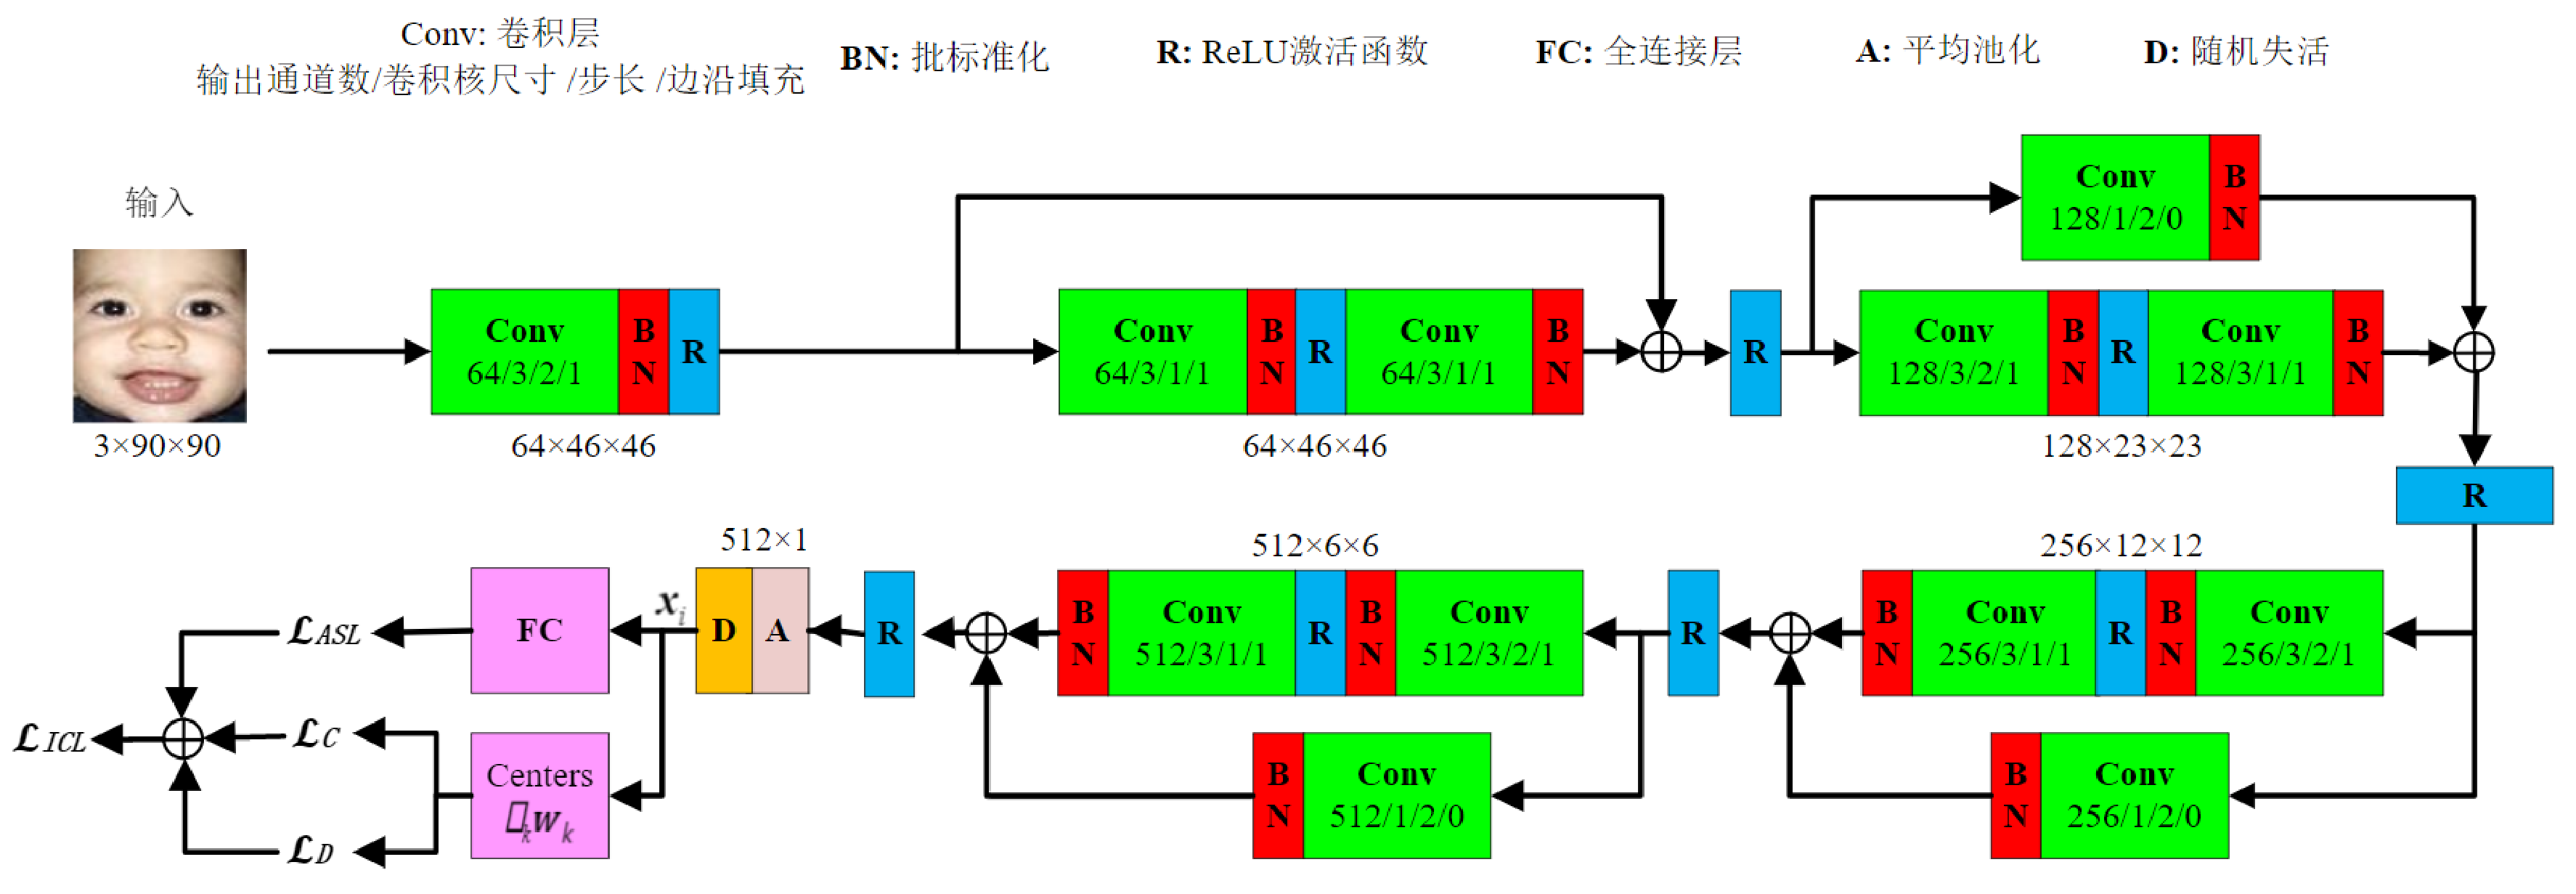
\includegraphics[height=5.63cm ,width=15.5cm]{figures/图4.1.eps}
	\caption{ICL损失函数仿真实验网络}\label{图4.1}
\end{figure}

(2)	实验数据集

实验采用四个非限制性分类数据集:AUCD2、FER2013、FERPlus和RAF-DB。

AUCD2数据集包含7名不同国家的31个驾驶人员的数据,AUCD2共有10个类别17303张图像,包括安全驾驶3686张、右手打字1974张、右手接电话1223张、左手打字1301张、左手接电话1361张、调收音机1220张、喝饮料1612张、拿后面东西1159张、整理头发和化妆1202张和与乘客交流2570张,拥有训练集标签和测试机标签文件。

FER2013数据集有7类表情共35886张图像,用于训练、验证和测试的图像分别是28709、3589和3589张。训练表情样本包括愤怒3995张、厌恶436张、恐惧4097张、悲伤4830张、开心7215张、惊讶3171张以及中性4965张。

FER2013中含有一些标注错误的数据,因而FERPlus数据集则对FER2013中的图像重新进行了人工标注,在FER2013的7类基本表情上又增加了蔑视、未知和非人脸三类。FERPlus每一张图像有10个分类标签,10个标签上的得分总和为10。本文只考虑7种基本表情,采用文献\cite{67}提供的最大投票方式筛选后的训练图像有24941张、验证图像3186幅、测试图像3137张。

RAF数据集拥有15339张表情图片,其中12271和3068分别用于训练和测试。训练图像含有的7类基本表情是愤怒705张、厌恶717张、恐惧281张、悲伤1982张、开心4772张、惊讶1290张以及中性2524张。

FER2013和FERPlus都含有验证集和测试集,本文只汇报测试集的测试结果。

(3)	图像预处理

AUCD2的图片是1920×1080的3通道彩色图,将其设置成100×100×3图片。FER2013和FERPlus的图片是48×48灰度图,先扩大成100×100图片,然后通过复制通道方式转换为100×100×3的图像。RAF-DB提供100×100×3的RGB彩色图像,无需转换。

训练时,从100×100×3人脸图像中随机剪切出90×90×3图像块,再把每一个像素值除以255归一化。为了增强数据,在±10°范围内随机旋转,且以50\%的概率随机水平翻转。

(4)	训练/测试策略

采用随机梯度下降法对模型进行端对端训练,每批128个表情样本,动量矩参数为0.9,采用的Heinitialization方法初始化卷积网络系数,L2正则系数为3×10-4,迭代次数为200,初始学习率为0.005,迭代80次后,每20代衰减率0.8。ICL的参数$\lambda_1$和$\lambda_2$分别为0.005和7。

测试阶段采用10-crop方法,100×100×3的图像被剪裁成10幅90×90×3的图像。



\subsection{性能评价标准}

本文采用文献\cite{66}中的平均准确率和稳定度两个标准。对每种方法测试$N(N=10)$次,以N次结果的平均值作为最终准确率,定义为:

\begin{equation}\label{公式4-12}
	Acc=\frac{\sum_{i=1}^{N}{Acc}_i}{N}
\end{equation}

${Acc}_i$是第$i$次实验的识别率。由于网络参数随机初始化和训练样本随机分批的原因,相同设置下每一次的识别结果有一定的误差,所以,采用多次实验的平均值更加公平可靠。

稳定度是$N$次实验结果的均方差,定义为:

\begin{equation}\label{公式4-13}
	S=\sqrt{\frac{\sum_{i=1}^{N}\left(Acc_i-Acc\right)^2}{N}}
\end{equation}

稳定度S体现了相同设置下实验结果的变化程度,S越小,表明模型性能越稳定。

\begin{table}[!ht]
	\caption{在AUCD2分类数据集上的性能比较}
	\label{表4.1}
	\renewcommand{\arraystretch}{1.5}
	\centering
	\begin{tabular}{p{3.5cm}<{\centering}p{3.5cm}<{\centering}p{3.5cm}<{\centering}}
		\bottomrule
		监督方法   & Acc(\%) & S \\ \hline
		SL     & 94.34                            & 0.532                      \\
		ASL    & 95.02                            & 0.428                      \\
		SL+CL  & 94.70                            & 0.634                      \\
		ASL+CL & 95.11                            & 0.563                      \\
		IL     & 94.21                            & 0.518                      \\
		L2SL   & 94.24                            & 0.564                      \\
		LP     & 95.13                            & 0.359                      \\
		ICL    & 95.87                            & 0.250                      \\ 
		\bottomrule
	\end{tabular}
\end{table}

\subsection{实验结果及分析}

(1)	表情识别性能对比

本文ICL是在SL基础上的改进,为了验证ICL的有效性,主要与SL及其改进技术进行对比,对比方法有:SL、ASL\cite{66}、SL+CL\cite{63}、ASL+CL、IL\cite{69}、L2SL\cite{68}和LP\cite{62}。


\begin{table}[!ht]
	\caption{在FER2013分类数据集上的性能比较}
	\label{表4.2}
	\renewcommand{\arraystretch}{1.5}
	\centering
	\begin{tabular}{p{3.5cm}<{\centering}p{3.5cm}<{\centering}p{3.5cm}<{\centering}}
		\bottomrule
		监督方法   & Acc(\%) & S     \\ 
		\hline
		SL     & 71.77   & 0.422 \\
		ASL    & 72.36   & 0.348 \\
		SL+CL  & 71.96   & 0.554 \\
		ASL+CL & 72.22   & 0.443 \\
		IL     & 71.53   & 0.428 \\
		L2SL   & 71.85   & 0.404 \\
		LP     & 72.25   & 0.339 \\
		ICL    & 73.02   & 0.210 \\ 
		\bottomrule
	\end{tabular}
\end{table}


本文在AUCD2、FER2013、FERPlus和RAF-DB四个数据集上进行了对比测试,为了公平对比,所有方法均采用图\ref{图4.1}中卷积网络,且采用相同的训练步骤和网络参数。ASL代码由原论文作者提供,其它方法则是按照文献所述原理另行编写程序。

\begin{table}[!ht]
	\caption{在FERPlus分类数据集上的性能比较}
	\label{表4.3}
	\renewcommand{\arraystretch}{1.5}
	\centering
	\begin{tabular}{p{3.5cm}<{\centering}p{3.5cm}<{\centering}p{3.5cm}<{\centering}}
		\bottomrule
		监督方法   & Acc(\%) & S     \\ 
		\hline
		SL     & 88.12   & 0.353 \\
		ASL    & 88.17   & 0.308 \\
		SL+CL  & 88.23   & 0.314 \\
		ASL+CL & 88.34   & 0.203 \\
		IL     & 88.15   & 0.281 \\
		L2SL   & 88.21   & 0.385 \\
		LP     & 88.38   & 0.276 \\
		ICL    & 88.56   & 0.192 \\ 
		\bottomrule
	\end{tabular}
\end{table}


在AUCD2数据集上的性能对表\ref{表4.1}所示,ICL的平均识别率Acc最高,达到了92.87\%,相比较于SL和ASL分别提高了1.53\%和0.85\%。在稳定度S方面,ICL也取得了最佳成绩0.250,相比较于SL的0.532,提高了一倍(注意:稳定度性能提升是指S的数值下降)。


在FER2013数据集上的性能对比结果如表\ref{表4.2}所示,ICL的平均识别率Acc最高,达到了73.02\%,比SL和ASL分别提高了1.25\%和0.66\%。在稳定度S方面,ICL也取得了最佳成绩0.210,相比于SL的0.422,提升了一倍。


\begin{table}[!ht]
	\caption{在RAF-DB分类数据集上的性能比较}
	\label{表4.4}
	\renewcommand{\arraystretch}{1.5}
	\centering
	\begin{tabular}{p{3.5cm}<{\centering}p{3.5cm}<{\centering}p{3.5cm}<{\centering}}
		\bottomrule
		监督方法   & Acc(\%) & S     \\ \hline
		SL     & 85.61   & 0.324 \\
		ASL    & 85.58   & 0.271 \\
		SL+CL  & 86.26   & 0.288 \\
		ASL+CL & 85.47   & 0.194 \\
		IL     & 85.49   & 0.182 \\
		L2SL   & 85.54   & 0.344 \\
		LP     & 86.11   & 0.247 \\
		ICL    & 86.26   & 0.180 \\ \bottomrule
	\end{tabular}
\end{table}


FERPlus数据集的测试结果如表\ref{表4.3}所示,在识别准确率和稳定度方面,ICL都取得了最好成绩,分别是88.56\%和0.192。相比于SL和ASL,ICL的准确度提高了0.44\%和0.39\%,其性能提升程度没有FER2013上显著。

RAF-DB数据集上的性能对比如表\ref{表4.4}所示,在识别准确度方面,SL+CL和ICL的识别率最高,达到88.26\%,但是ICL的稳定度是0.180,要比SL+CL的稳定度0.288好得多。


从表\ref{表4.1}-\ref{表4.4}可知,总体而言,ASL优于SL,SL+CL也很优秀,但是ASL+CL在FER2013数据库上的识别率和稳定性都比ASL差,在RAF-DB数据集上识别率也低于ASL,说明ASL+CL可能比单独的ASL更差,这也是本文提出ICL的出发点。ICL是以ASL为基础,融合了CL的思想,再加入了最大化类间空间距离的思想,ICL在三个数据库上都表现优异,表明了ICL的合理性和有效性。

\begin{figure}[!ht]
	\centering
	\subfloat[$\lambda_2=7$,$\lambda_1$变化]{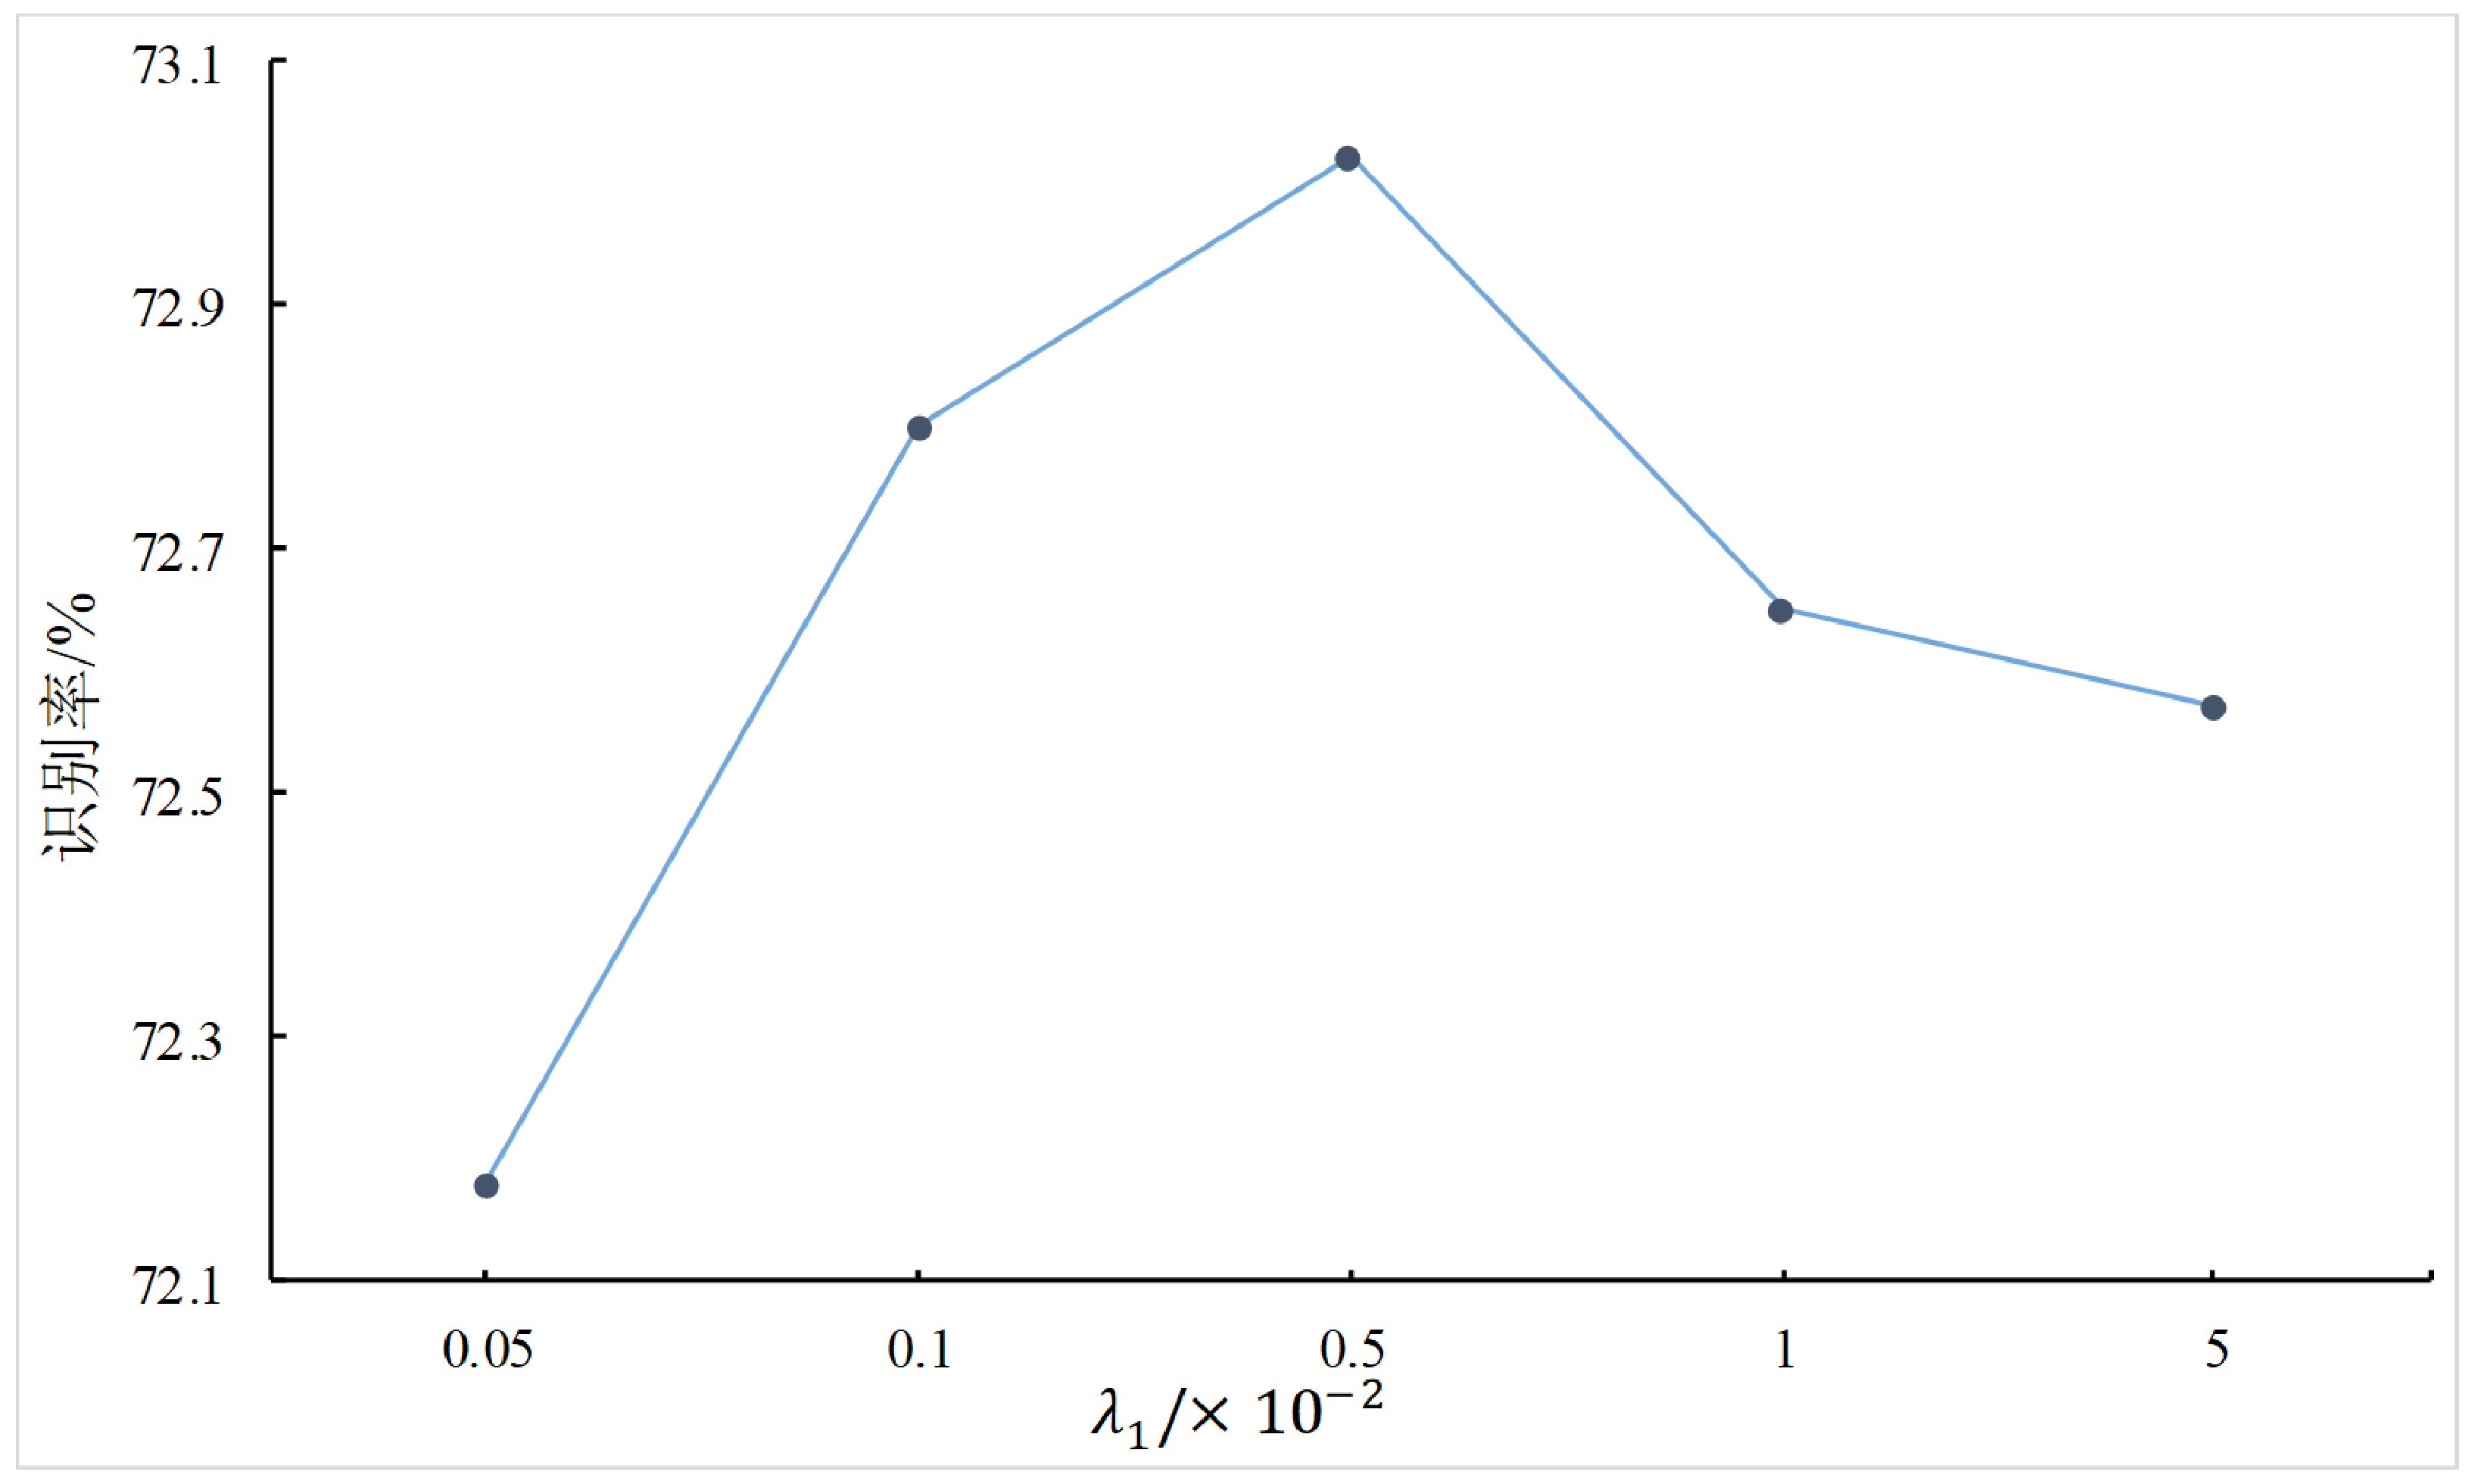
\includegraphics[height=6.22cm, width=10.44cm]{figures/图4.2a.eps}%
	}
	\hfil
	\subfloat[$\lambda_1=0.005$,$\lambda_2$变化]{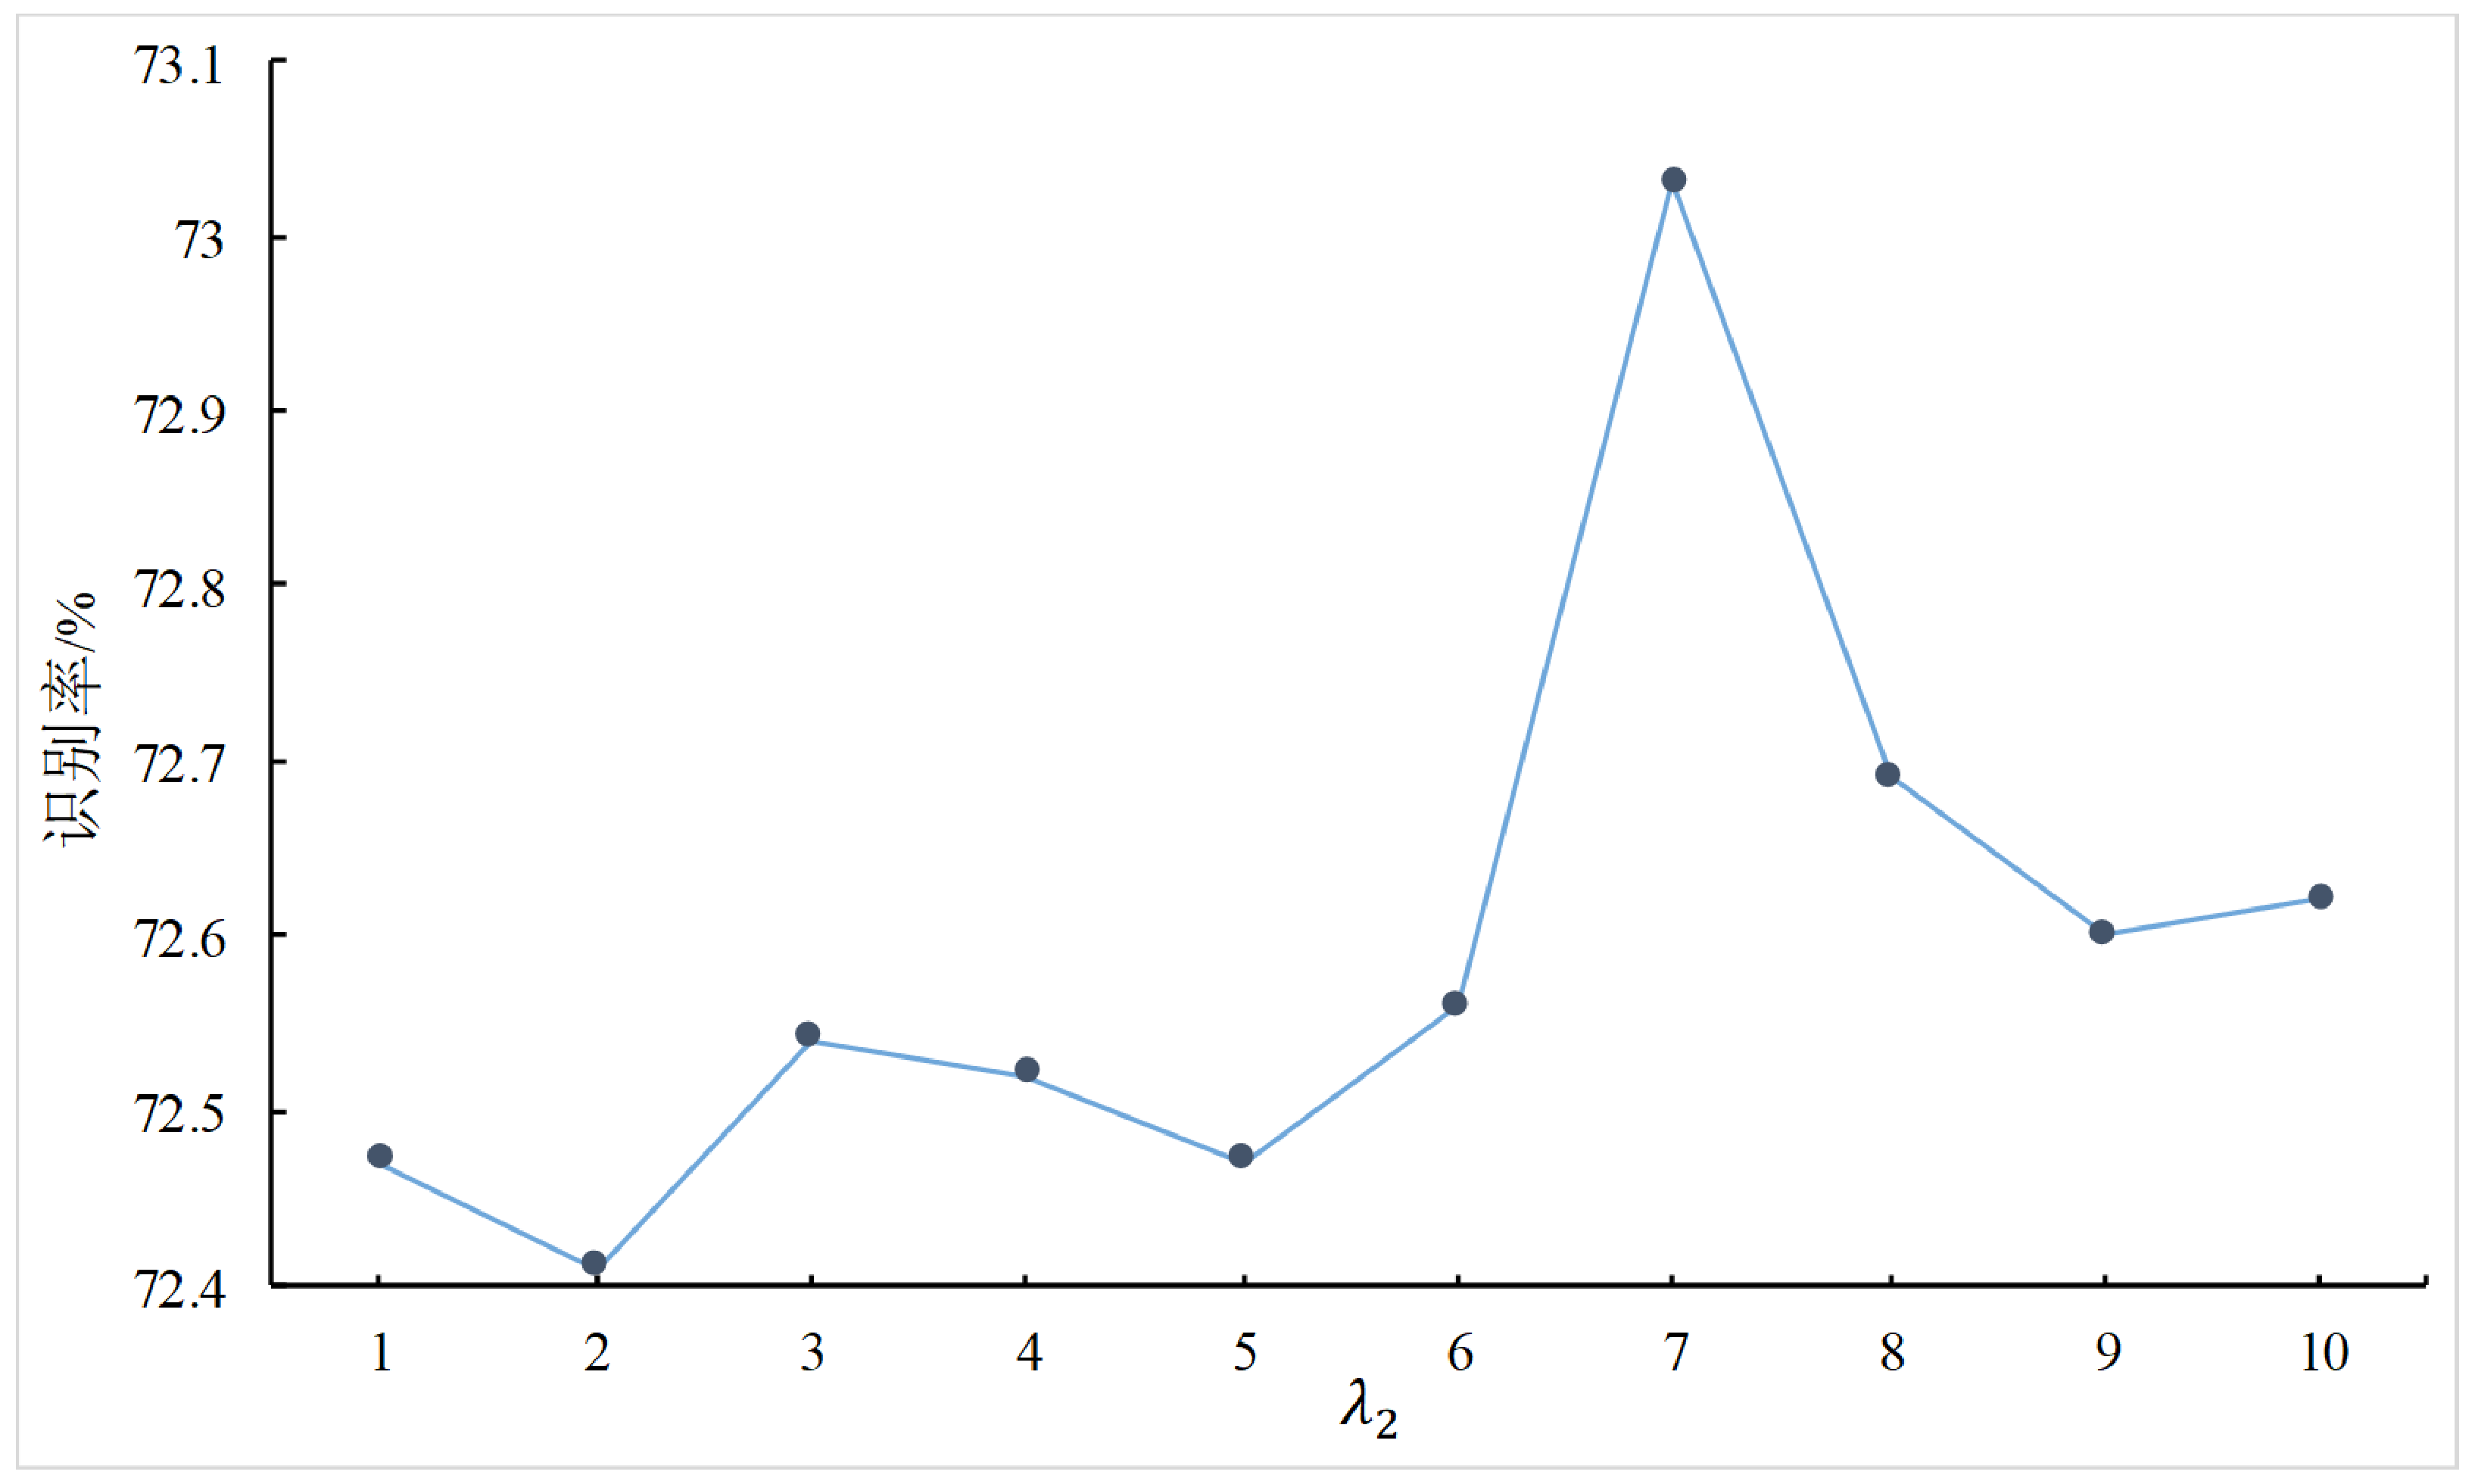
\includegraphics[height=6.22cm, width=10.44cm]{figures/图4.2b.eps}%
	}
	\caption{设置不同参数设置$\lambda_1$和$\lambda_2$在FER2013上的准确率}
	\label{图4.2}
\end{figure}

(2)	参数选择

ICL有两个人为设置的权值$\lambda_1$和$\lambda_2$(见公式\ref{公式4-9}),理论上应该采用网格计算最优权值。文献\cite{63,64,69,61}表明减小类内变化的约束权值在0.001~0.01区间比较合理,因而本文首先设置$\lambda_1$为0.005,然后$\lambda_2$取1到10共10个值,在FER2013数据集上的识别准确率如图\ref{图4.2}(b)所示,虽然不是严格的上凸曲线,整体而言,$\lambda_2=7$时的识别率明显优于其它值。

$\lambda_2$设置为7,然后$\lambda_1$分别取值0.0005、0.001、0.005、0.01及0.05共5个值,在FER2013数据集上的识别结果如图\ref{图4.2}(a)所示,能够明显地观察到,$\lambda_1=0.005$时的识别率最高。

综上所述,本文选取$\lambda_1=0.005$和$\lambda_2=7$。


% Please add the following required packages to your document preamble:
% \usepackage{multirow}
\begin{table}[!ht]
	\caption{消融实验}
	\centering
	\renewcommand{\arraystretch}{1.5}
	\label{表4.5}
	\begin{tabular}{p{2.75cm}<{\centering}p{1.25cm}<{\centering}p{1.25cm}<{\centering}p{1.25cm}<{\centering}p{1.25cm}<{\centering}p{1.25cm}<{\centering}p{1.25cm}}
		\bottomrule
		\multirow{2}{*}{监督方法}                                                                                 & \multicolumn{2}{c}{FER2013} & \multicolumn{2}{c}{FERPlus} & \multicolumn{2}{c}{RAF-DB} \\ \cline{2-7} 
		& Acc/\%        & S           & Acc/\%        & S           & Acc/\%       & S           \\ \hline
		$\mathcal{L}_{ASL}$                                                               & 72.36         & 0.348       & 88.17         & 0.308       & 85.58        & 0.271       \\
		$\mathcal{L}_{ASL}+\mathcal{L}_C$                                & 72.23         & 0.188       & 88.47         & 0.167       & 85.89        & 0.187       \\
		$\mathcal{L}_{ASL}+\mathcal{L}_C+\mathcal{L}_D$ 				 & 73.02         & 0.210       & 88.56         & 0.192       & 86.26        & 0.180       \\ \bottomrule
	\end{tabular}
\end{table}


(3)	消融实验

ICL损失函数由三部分构成:ASL损失$\mathcal{L}_{ASL}$、类内损失$\mathcal{L}_C$(公式4-7)和类间距离损失$\mathcal{L}_D$(公式\ref{公式4-8}),本次消融实验测试了$\mathcal{L}_{ASL}$(ASL)、$\mathcal{L}_{ASL}+\mathcal{L}_C$和$\mathcal{L}_{ASL}+\mathcal{L}_C+\mathcal{L}_D$(ICL),其结果如表\ref{表4.5}所示(这里的$\mathcal{L}_{ASL}+\mathcal{L}_C$与对比实验中的ASL+CL是不同的方法)。


在FER2013数据库上,$\mathcal{L}_{ASL}$的识别率和稳定度分别是72.36\%和0.348。加入$\mathcal{L}_C$损失($\mathcal{L}_{ASL}+\mathcal{L}_C$)后则分别是72.23\%和0.188,识别率反而略微下降,但是稳定度性能大幅提升。再加入$\mathcal{L}_D$($\mathcal{L}_{ASL}+\mathcal{L}_C+\mathcal{L}_D$)后的成绩分别是73.02\%和0.210,$\mathcal{L}_{ASL}+\mathcal{L}_C+\mathcal{L}_D$在识别率方面有了明显的提高;在稳定性方面,比$\mathcal{L}_{ASL}+\mathcal{L}_C$的稳定度稍差一点,但仍然比$\mathcal{L}_{ASL}$优秀很多。

在FERPlus数据集中,$\mathcal{L}_{ASL}$、$\mathcal{L}_{ASL}+\mathcal{L}_C$和$\mathcal{L}_{ASL}+\mathcal{L}_C+\mathcal{L}_D$三种方式的识别率分别是88.17\%、88.47\%和88.56\%,依次略微提升。这三种方式的稳定度分别是0.308、0.167和0.192,$\mathcal{L}_{ASL}+\mathcal{L}_C$的稳定度好,$\mathcal{L}_{ASL}+\mathcal{L}_C+\mathcal{L}_D$的稳定度反而比$\mathcal{L}_{ASL}+\mathcal{L}_C$稍微差一点,但比$\mathcal{L}_{ASL}$仍然好很多。

在RAF-DB数据库上,$\mathcal{L}_{ASL}$、$\mathcal{L}_{ASL}+\mathcal{L}_C$和$\mathcal{L}_{ASL}+\mathcal{L}_C+\mathcal{L}_D$的识别准确率分别是85.58\%、85.89\%和86.26\%,依次增高。三者的稳定度分别是0.271、0.187和0.180,也是依次变好;$\mathcal{L}_{ASL}+\mathcal{L}_C$和$\mathcal{L}_{ASL}+\mathcal{L}_C+\mathcal{L}_D$的稳定度非常接近,几乎差不多。

由此可见,大体上,$\mathcal{L}_{ASL}+\mathcal{L}_C$可以大幅增加稳定性,$\mathcal{L}_{ASL}+\mathcal{L}_C+\mathcal{L}_D$在保持稳定性优势的基础上可以提高一定的识别准确度。

(4)	时间复杂度

各种监督方法在FER2013数据集上训练一个Epoch所需的平均时间如表\ref{表4.6}所示,ASL速度最快,只需33.51秒。SL是33.92秒,ASL+CL与SL几乎差不多,需要33.97秒。ICL是以ASL为基础融合了CL思想,再增加了一部分约束,所以ICL比ASL+CL计算复杂度高,需要34.31秒,仍然比SL+CL略微快一点,比IL和L2SL快很多。

\begin{table}[!ht]
	\caption{FER2013数据集上训练一个Epoch所需平均时间(单位:秒)}
	\label{表4.6}
	\renewcommand{\arraystretch}{1.5}
	\centering
	\begin{tabular}{p{2cm}<{\centering}p{1.25cm}<{\centering}p{1.25cm}<{\centering}p{1.25cm}<{\centering}p{1.25cm}<{\centering}p{1.25cm}<{\centering}p{1.25cm}<{\centering}p{1.25cm}<{\centering}}
		\bottomrule
		监督方法  & SL    & ASL   & SL+CL & ASL+CL & IL    & L2SL  & ICL   \\ \hline
		时\ \ 间 & 33.92 & 33.51 & 34.38 & 33.97  & 42.15 & 36.36 & 34.31 \\ \bottomrule
	\end{tabular}
\end{table}

\section{本章小节}


本章的主要内容包含以下几部分:

(1)	本章节从分类任务的目的性出发,阐述了分类任务中,作为重点的分类器在类别特征区分上存在的问题,即SL损失函数区分度过度依赖样本呢均衡,对不平衡数据集出现样本数量多类别对样本数量少类别类别在样本特征角度域空间中挤压的问题。进而介绍了多种克服挤压问题方法的优势和不足,引出了本章改进此问题孤立中心损失函数(ICL)的必要性。

(2)	针对传统SL监督学习的深度特征区分度不足问题,提出了一种孤立中心损失方法(ICL),它主要包含了最大化类间角度距离、减小类内变化以及最大化类间(欧氏)空间距离三种约束,从而使各类成为彻底的“孤岛”,以提高各类之间的区分度。

(3)	在AUCD2、FER2013、FERPlus和RAF-DB四个数据集上的实验结果表明:ICL在识别准确率和稳定性两个方面都有明显的提升。ICL虽然由三部分组成,但是计算复杂度并未增加太多,运行速度只比传统SL略微慢一点,仍然比一些其它方法快。

(4) ICL的基础是ASL,ASL中生成等角分布固定权值向量过程的计算量随着类别数量增大而呈几何形式增长,难以处理类别特别多的分类任务,所以,ICL仍然需要进一步去解决这个问题。







